\chapter{总体设计}
\section{软件描述}
系统包括前台和后台两个部分。

\subsection{前台主要功能}
\indent    发送请求并接收服务器的响应,对返回结果进行渲染展示。\\
\indent    对于用户而言,为用户在web端提供一套完整的旅行服务,从用户出行的航班、火车票预订到酒店预订,景点推荐和门票预订,用户在登录帐号后可以和服务器建立通信关系,用户通过前端的展示进行选择或者输入提交,产生发送对应的请求与动作,接收服务器端的响应。\\
\indent    对于管理员而言,在登录到前端的管理系统后,可以看活动、门票、航班和用户等所有的信息,web前端可以方便管理员高效管理,管理员可以通过每一种类(如火车票/航班等)的新建选项发布新的信息,或者通过编辑修改信息。
\subsection{后台主要功能}
\indent    接收用户/管理员在web端发送的动作和请求,处理并响应。\\
\indent    服务器在接收到用户请求时,会在服务器的数据库中进行查询操作,并且进行返回查询结果或者反馈提示信息,对于用户提交的数据(比如预订、编辑个人信息),也会存入到数据库中。\\
\indent    服务器在接收到管理员的提交时,会在数据库中插入数据记录进行更新。

\newpage
\section{处理流程}
\subsection{总体流程}
说明:该流程图为旅行管理系统的宏观展示,用户和管理员为该系统的两个活动角色,基于旅行服务管理系统,用户从系统中获取旅行相关的各种信息,而管理员负责维护该系统,并且管理用户,为用户提供全方位的优质服务。
\begin{figure}[ht]
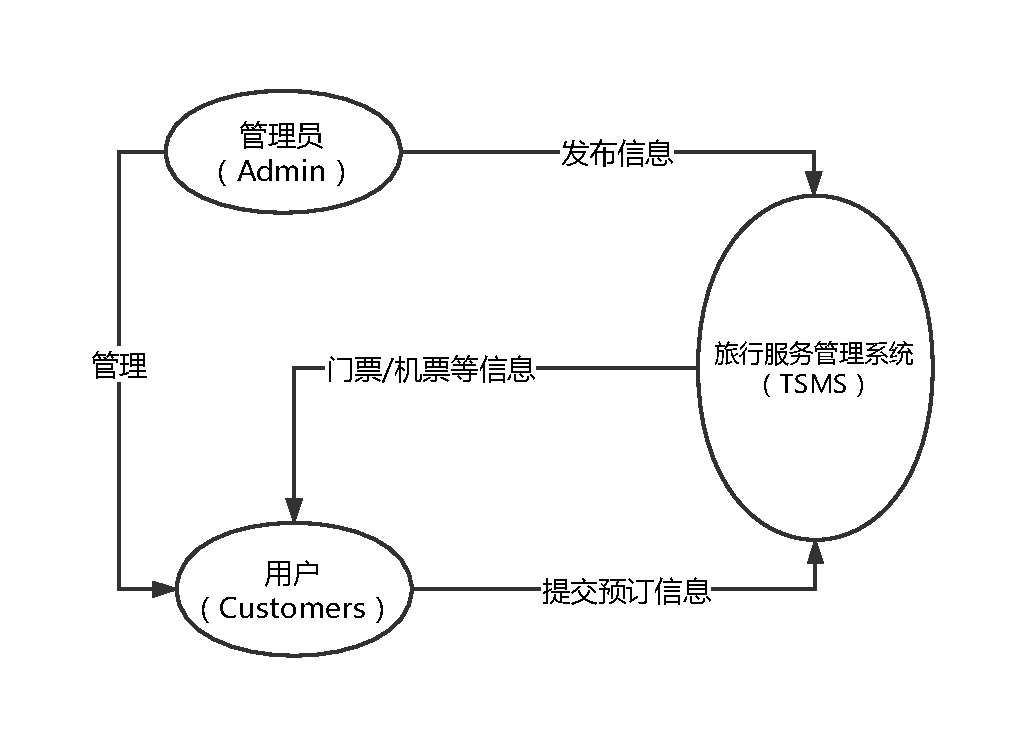
\includegraphics[width=16cm]{process2}
\caption{系统基本流程} \label{fig:figure2}
\end{figure}

\subsection{系统基本流程}
说明:该流程图为旅行管理系统的整个工作流程,其中蓝色字体所示是以用户需求为例的请求——响应流程,橙色字体所示是以管理员发布信息为例的发布——更新流程。(实际中用户也会提交更新请求,管理员也会有查询请求)
\newpage

\begin{figure}[htbp]
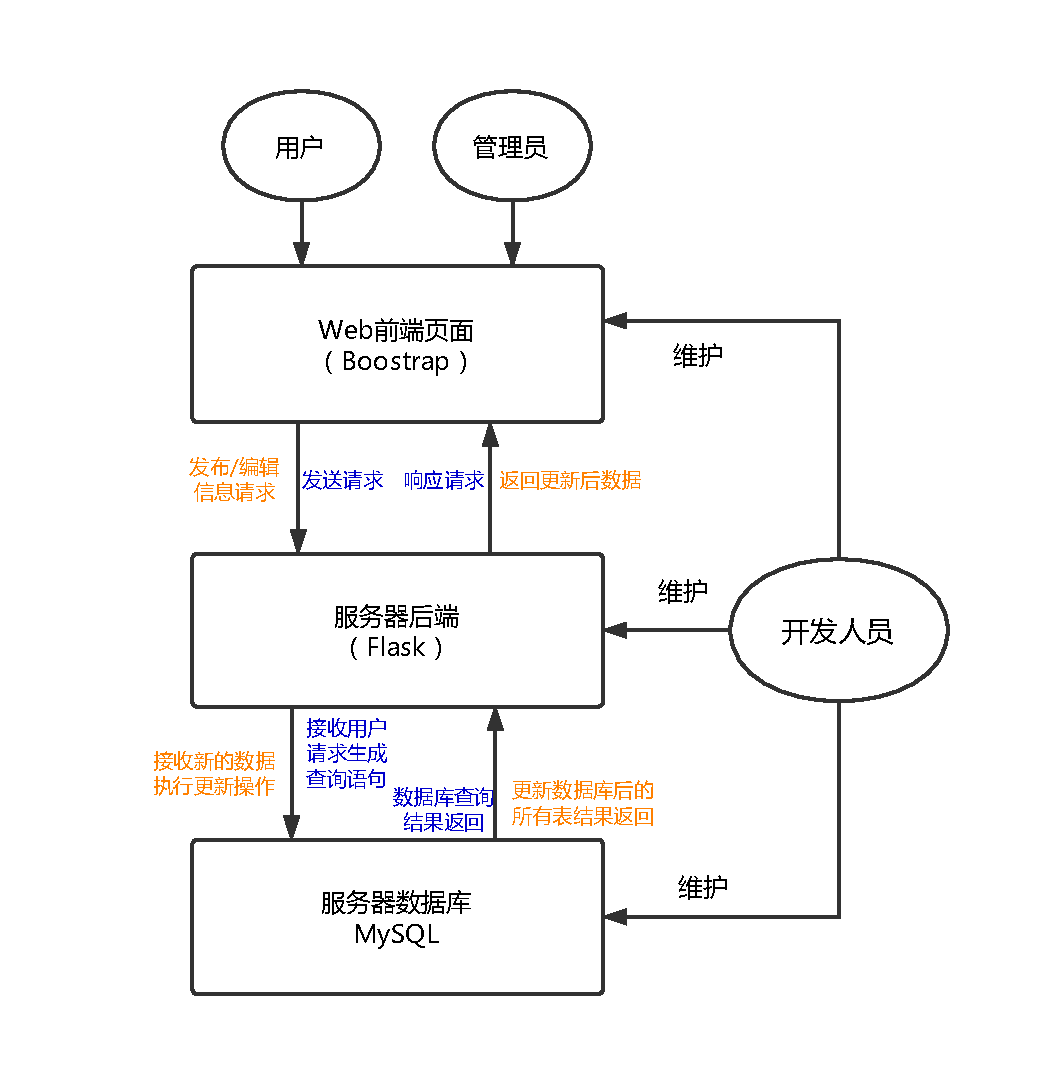
\includegraphics[width=16cm]{process1}
\caption{系统基本流程} \label{fig:figure1}
\end{figure}

\subsection{客户端基本流程}
说明:用户或者管理员在浏览器中输入用户名和密码进行验证登录(如果没有用户名需要先注册),登录后的web前端界面首页显示为广告活动的推送,前端为管理员(登录id验证为1)提供了广告活动、航班、火车票、酒店、景点门票以及优惠券的发布和编辑选项,为用户提供了航班、火车票、酒店和景点门票的预订选项,同时可以领取优惠券享受相应的折扣,用户也可以与客服在线即时沟通,用户的预订行为会作为输入提供给推荐算法为用户进行个性化的推荐。
\begin{figure}[htbp]
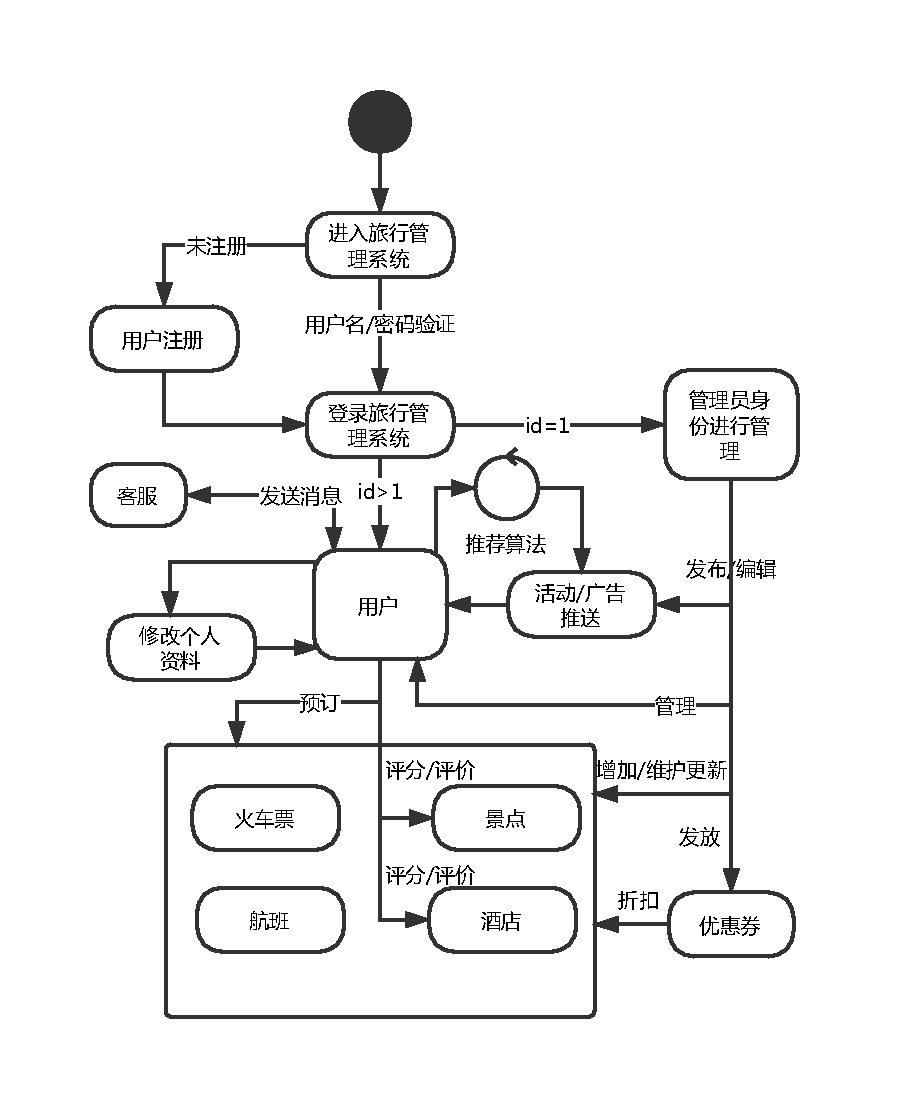
\includegraphics[width=18cm]{process3}
\caption{客户端基本流程} \label{fig:figure3}
\end{figure}

\subsection{服务器端基本流程}
说明:服务器端的nginx通过80端口与web客户端进行通信,在收到航班、火车票、酒店和景点的查询请求时反向代理把请求转发给WSGI服务器gunicorn,后者接收到请求后直接在flask后端的逻辑控制模块生成sql查询语句连接到数据库,完成查询操作后按照原路返回到80端口。更新/提交请求也是类似的处理过程,在下图都有说明。优惠券和活动无需查询操作,直接返回到客户端。用户消息转发到WSGI服务器后把消息发送给客服,并接受客服消息转发给客户。

\begin{figure}[htbp]
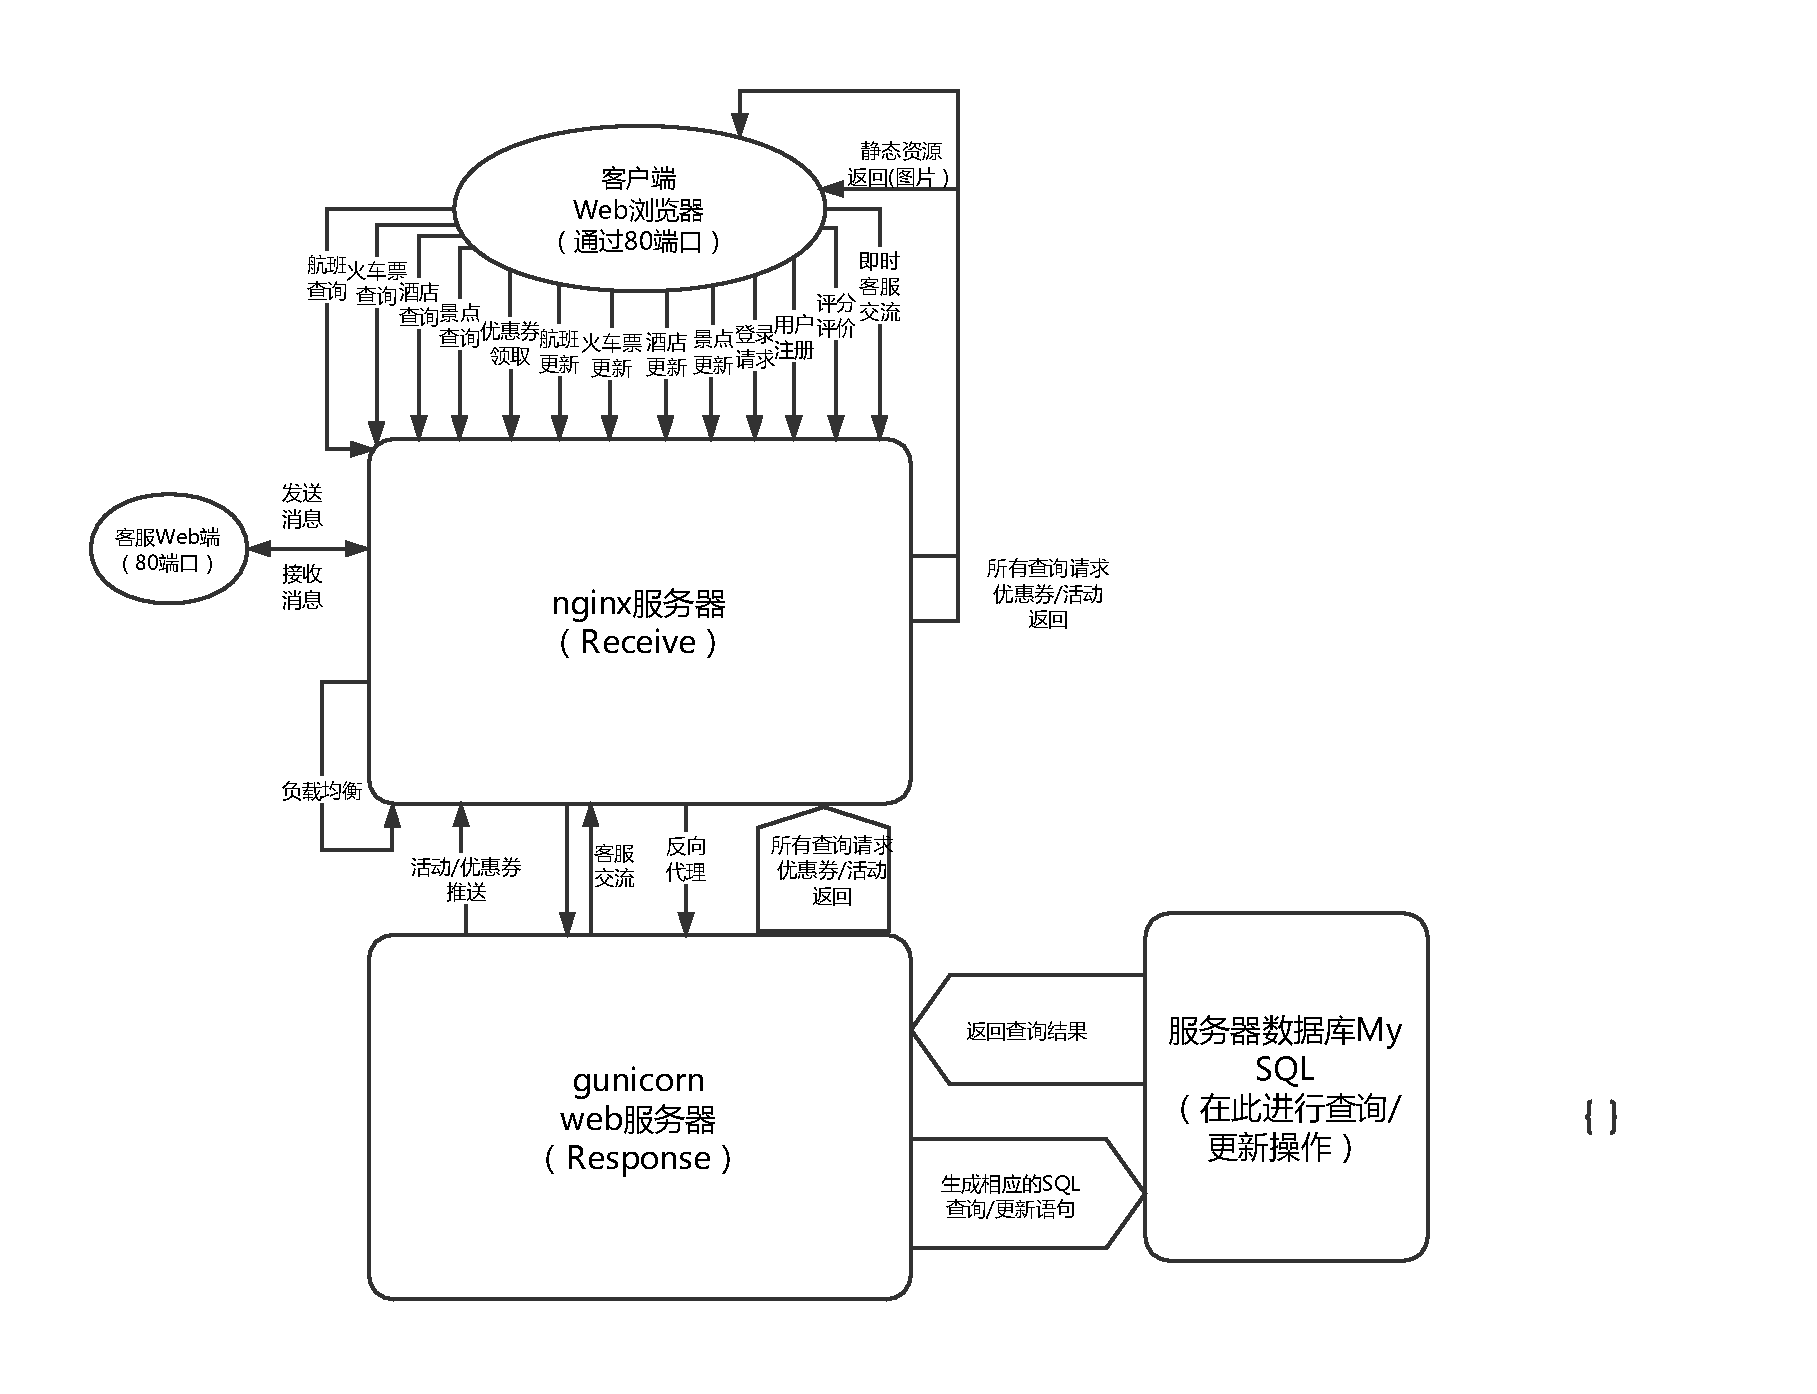
\includegraphics[width=22cm]{process4}
\caption{服务器端基本流程} \label{fig:figure4}
\end{figure}

\subsection{功能1——注册和登录验证具体流程}
用户如果没有登录系统,在web前端的上方菜单栏会有注册和登录两个选项。注册时用户在注册界面填写注册信息,提交后生成表单作为Post请求发送给服务器,服务器接收到注册提交请求后,首先根据输入用户名在后端数据库中查询,如果查询返回不为空,说明该用户名已被注册,返回给用户提示信息"用户名已经存在",之后会检测输入的两次密码是否一致,确实无误后将用户信息插入到数据库完成注册。用户登录时提交post请求,服务器端查询数据库判断该用户名是否存在以及密码是否正确,通过后用户登录,创建session对话。

\subsection{功能2——用户预订/领取具体流程}
已经登录的用户(id>1)可以从web前端看到所有的航班/火车票/酒店/景点信息,同时种类的每一个项目都有预订选项,用户点击预订后提交请求,服务器端接收数据并更新数据库,然后返回给用户当前预订的数量,并且增加了取消预订的选项。优惠券的领取流程与上述类似,当某个优惠券用户未领取时可以点击领取按钮提交请求,服务器将优惠券信息更新到数据库。

\subsection{功能3——用户提交评论具体流程}
在使用优惠券之后可以发表对酒店/景点的评分,用户可以提交一个1-5分的浮点数评分和小于100个字符的评论,生成表单并提交post请求,服务器端接收数据并且将评论信息插入到数据库。

\subsection{功能4——管理员发布信息具体流程}
在管理员登录后(id=1)可以从web前端对所有类别的预订项目进行管理,在每一个类别(航班/机票/火车票/门票)下都可以新建或者编辑条目,提交后服务器端接收post请求并且将相应的记录更新到数据库以供用户查询。同时管理员亦可以在网页的首页发布新的活动,以及发放新的优惠券,提交到服务器的流程类似。

\subsection{功能5——客户服务具体流程}
在用户登录之后在个人的菜单栏有客服这一选项,用户可以在线输入信息并且发送,服务器接收消息数据并且转发给相关客服人员,客服回复之后类似的通过服务器发送回用户的前端,从而实现即时通讯,这一过程无需经过数据库。

\subsection{功能6——个性化推荐系统具体流程}
对于已经登录的用户,在服务器端推送活动时,会查询到用户相关的历史预订信息以及评论,从而可以判断用户的旅行喜好和个性化特点,同时也会进行用户间的相似度匹配,如果与某个用户相似度很高,那么另一个用户的相关记录可以作为依据将活动推送给该用户,整个流程为将用户个人数据集作为输入交给推荐算法进行处理,并结合后台数据库,从而生成个性化的推荐结果。




\section{功能结构设计}
\subsection{整体结构}
旅行服务管理系统的整体结构为Web前端——服务器——Mysql数据库架构,这三个子系统可以相邻的进行通信,三个层次的开发架构便于管理和维护,每个子系统的结构会分别详细说明。
\begin{figure}[htbp]
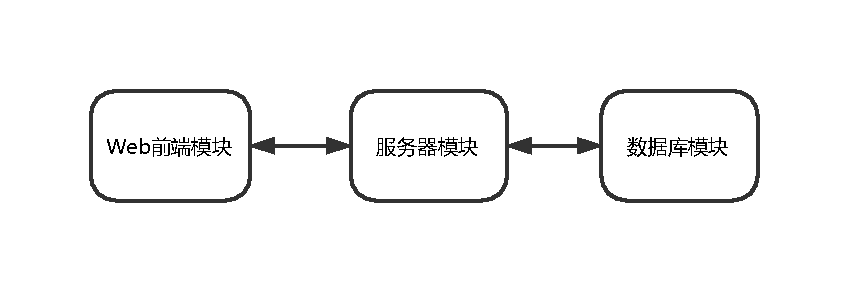
\includegraphics[width=18cm]{struct1}
\caption{整体结构} \label{fig:figure5}
\end{figure}

\subsection{用户端结构}
在web前端的设计中,需要展现给用户的是一个美观且结构化的界面,所以在用户端的结构设计中,对每一个种类的模块进行具体划分,每一个模块都在前端网页的顶部菜单栏中找到对应的入口选项,并且为下图所示的模块都独立开发操作和展示界面,便于用户进行选择和提交。
\begin{figure}[htbp]
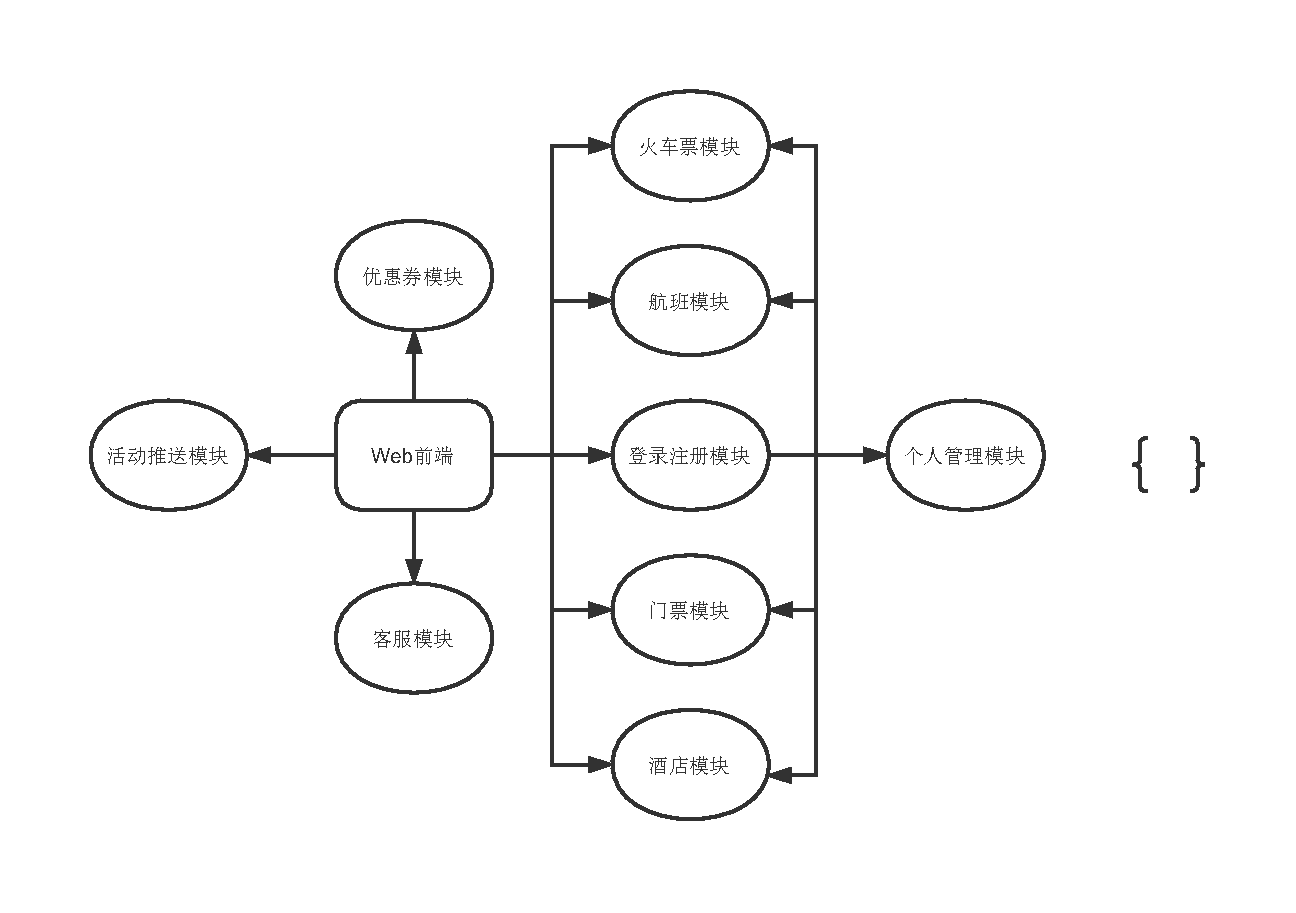
\includegraphics[width=22cm]{struct2}
\caption{用户端结构} \label{fig:figure6}
\end{figure}

\subsection{服务器端结构}
服务器作为整个管理系统的核心,其分别设有前端交互的接口模块和与后端数据库进行通信的模块,同时整个系统的逻辑控制都是在服务器中进行,并且针对用户特定需求增加了个性化的推荐模块,通过有效的推荐算法为用户提供更加优质的推荐。
\begin{figure}[htbp]
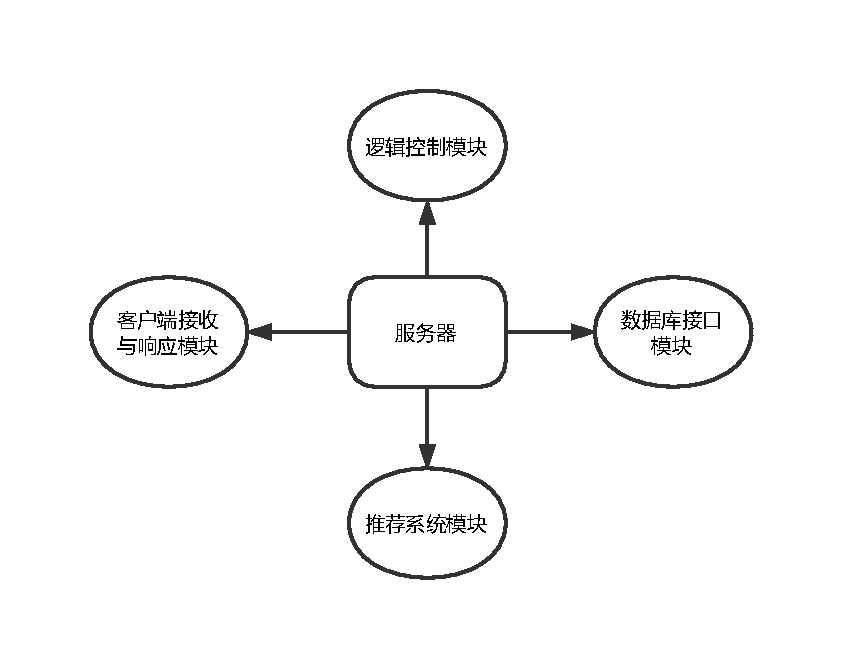
\includegraphics[width=16cm]{struct3}
\caption{服务器端结构} \label{fig:figure7}
\end{figure}

\subsection{后台数据库维护模块结构}
数据库模块需要接收来自于服务器的查询和更新请求,在数据库的设计中针对用户需求设有如下图所示的多个表结构,层次清晰便于进行数据库的维护管理。
\begin{figure}[htbp]
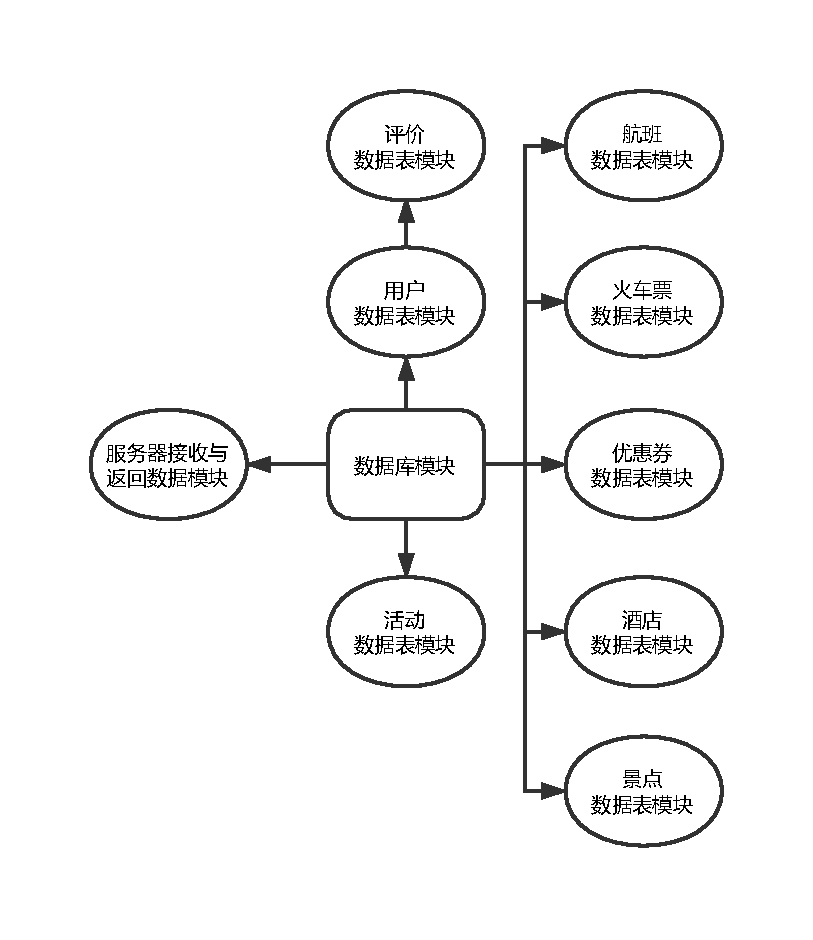
\includegraphics[width=16cm]{struct4}
\caption{后台数据库维护模块结构} \label{fig:figure8}
\end{figure}


\section{功能需求与程序代码的关系}
[此处指的是不同的需求分配到哪些模块去实现。可按不同的端拆分此表]
\begin{table}[htbp]
\centering
\caption{功能需求与程序代码的关系表} \label{tab:requirement-module}
\begin{tabular}{|c|c|c|c|c|c|c|c|}
    \hline
    · & 酒店模块 & 火车票模块 & 航班模块 & 景点模块 & 登录注册模块 & 优惠券模块 \\
    \hline
    酒店预订 & Y & · & · & · & Y & Y \\
    \hline
    火车票预订 & · & Y & · & · & Y & Y \\
    \hline
    机票预订 & · & · & Y & · & Y & Y \\
    \hline
    门票预订 & · & · & · & Y & Y & Y \\
    \hline
    广告/活动推送 & · & · & · & · & Y & · \\
    \hline
    优惠券 & · & · & · & · & Y & Y \\
    \hline
    用户登录 & · & · & · & · & Y & · \\
    \hline
    注册/修改信息 & · & · & · & · & Y & · \\
    \hline


\end{tabular}
\begin{tabular}{|c|c|c|c|c|c|c|c|}
    \hline
    · & 活动推送模块 & 客服模块 & 推荐系统 & 数据库模块 & NULL & NULL \\
    \hline
    酒店预订 & · & · & Y & Y & · & · \\
    \hline
    火车票预订 & · & · & Y & Y & · & · \\
    \hline
    机票预订 & · & · & Y & Y & · & · \\
    \hline
    门票预订 & · & · & Y & Y & · & · \\
    \hline
    广告/活动推送 & Y & · & Y & Y & · & · \\
    \hline
    用户评价 & · & Y & · & Y & · & · \\
    \hline
    优惠券 & · & · & · & Y & · & · \\
    \hline
    客户服务 & · & Y & · & · & · & · \\
    \hline
    用户登录 & · & · & · & Y & · & · \\
    \hline
    注册/修改信息 & · & · & · & Y & · & · \\
    \hline
\end{tabular}
\note{各项功能需求的实现与各个程序模块的分配关系}
\end{table}